\documentclass[conference]{IEEEtran}

\usepackage{amsmath}
\usepackage{booktabs}
\usepackage{graphicx}
\usepackage{xcolor}
\usepackage{soul}
\usepackage{url}

\graphicspath{{assets/}}
\DeclareGraphicsExtensions{.png,.jpg,.jpeg,.pdf}

\title{KLERT: Explainable Medical AI and DICOM Progression System for Brain MRI Analysis}

\author{
\IEEEauthorblockN{Anandita Indurkhya}
\IEEEauthorblockA{
Department of Computer Science and Engineering (AIML)\\
Shri Shankaracharya Institute of Professional Management and Technology, Raipur, India}
\thanks{Prepared for CMES 2027, the IEEE Guwahati Subsection's International Conference on Medical Engineering and Science, to be held February 11--13, 2027, at IIT Guwahati, Assam.}
}

\begin{document}
\bstctlcite{IEEEexample:BSTcontrol}
\maketitle

\begin{abstract}
Brain MRI interpretation requires both accurate classification and clinically meaningful evidence. This paper presents KLERT, an explainable medical artificial intelligence system that combines three image-classification models, Grad-CAM visual explanations, longitudinal three-dimensional DICOM progression analysis, and automated clinical-summary generation in one web application. The system evaluates a custom BrainTumorCNN, ResNet-18, and VGG-16 on four classes: glioma, meningioma, no tumor, and pituitary tumor. In the project evaluation, the custom model achieved 95.82\% accuracy, compared with 93.94\% for ResNet-18 and 92.25\% for VGG-16. The DICOM module estimates tumor volume from voxel dimensions and segmentation masks, while the interface presents predictions, confidence scores, heatmaps, and historical volume change together. KLERT is intended as an educational and research decision-support prototype; it does not replace radiological diagnosis or clinical validation.
\end{abstract}

\begin{IEEEkeywords}
brain MRI, explainable artificial intelligence, Grad-CAM, DICOM, longitudinal analysis, medical image classification, FastAPI
\end{IEEEkeywords}

\section{Introduction}
Magnetic resonance imaging (MRI) is central to brain-tumor assessment because it provides strong soft-tissue contrast without ionizing radiation. Manual review of multi-slice studies is time-consuming and can vary between observers, while many computer-aided diagnosis systems provide only an opaque class label. A useful research system should expose model evidence, compare alternative models, and preserve information about change across visits.

KLERT addresses these requirements through an integrated workflow for brain MRI classification and longitudinal progression analysis. The system combines a custom convolutional neural network (CNN) with pretrained ResNet-18 and VGG-16 models, generates Grad-CAM heatmaps, reads compatible DICOM series and tumor masks, and returns structured results through a FastAPI service. The project makes the following contributions:
\begin{itemize}
\item a consistent multi-model inference pipeline for four brain MRI classes;
\item visual explanations linked to the input image and selected model;
\item three-dimensional tumor-volume estimation and visit-to-visit comparison; and
\item a web workflow that combines analysis, comparison, testing, and clinical-summary features.
\end{itemize}

\section{Related Work}
Deep CNNs have become an important foundation for medical-image analysis, but performance alone does not establish clinical usefulness. ResNet introduced residual connections that support deeper networks \cite{he2016resnet}, while VGG demonstrated the value of small convolutional filters in visual recognition \cite{simonyan2015vgg}. Reviews of medical-image deep learning emphasize the need for careful validation, representative datasets, and awareness of domain shift \cite{litjens2017survey}.

Grad-CAM explains a class prediction by weighting late convolutional feature maps according to their gradients \cite{selvaraju2017gradcam}. DICOM provides the metadata and pixel-data conventions needed to represent medical imaging studies and their acquisition context \cite{dicom2024}. KLERT combines these established components with longitudinal volume calculations and a user-facing application rather than treating classification as an isolated benchmark.

\section{Problem Statement and Objectives}
The project targets four practical limitations:
\begin{enumerate}
\item single-model systems may provide unstable or difficult-to-audit predictions;
\item black-box predictions do not show which image regions influenced the result;
\item isolated-scan analysis does not reveal tumor growth or shrinkage over time; and
\item technical model outputs are difficult to use without a coherent interface and report format.
\end{enumerate}

Accordingly, KLERT aims to classify MRI scans, expose confidence distributions, generate spatial explanations, calculate three-dimensional progression metrics, and present the results through a reproducible web workflow. The output is a research aid and must be interpreted by a qualified professional.

\section{System Analysis and Architecture}
KLERT follows a layered architecture. The browser interface manages image selection, model selection, comparison controls, result cards, and visual overlays. The FastAPI layer validates requests and coordinates inference. Model modules load the trained weights and return class probabilities. Utility modules perform image transformation, Grad-CAM generation, DICOM parsing, volume computation, and report formatting.

\begin{figure}[t]
\centering
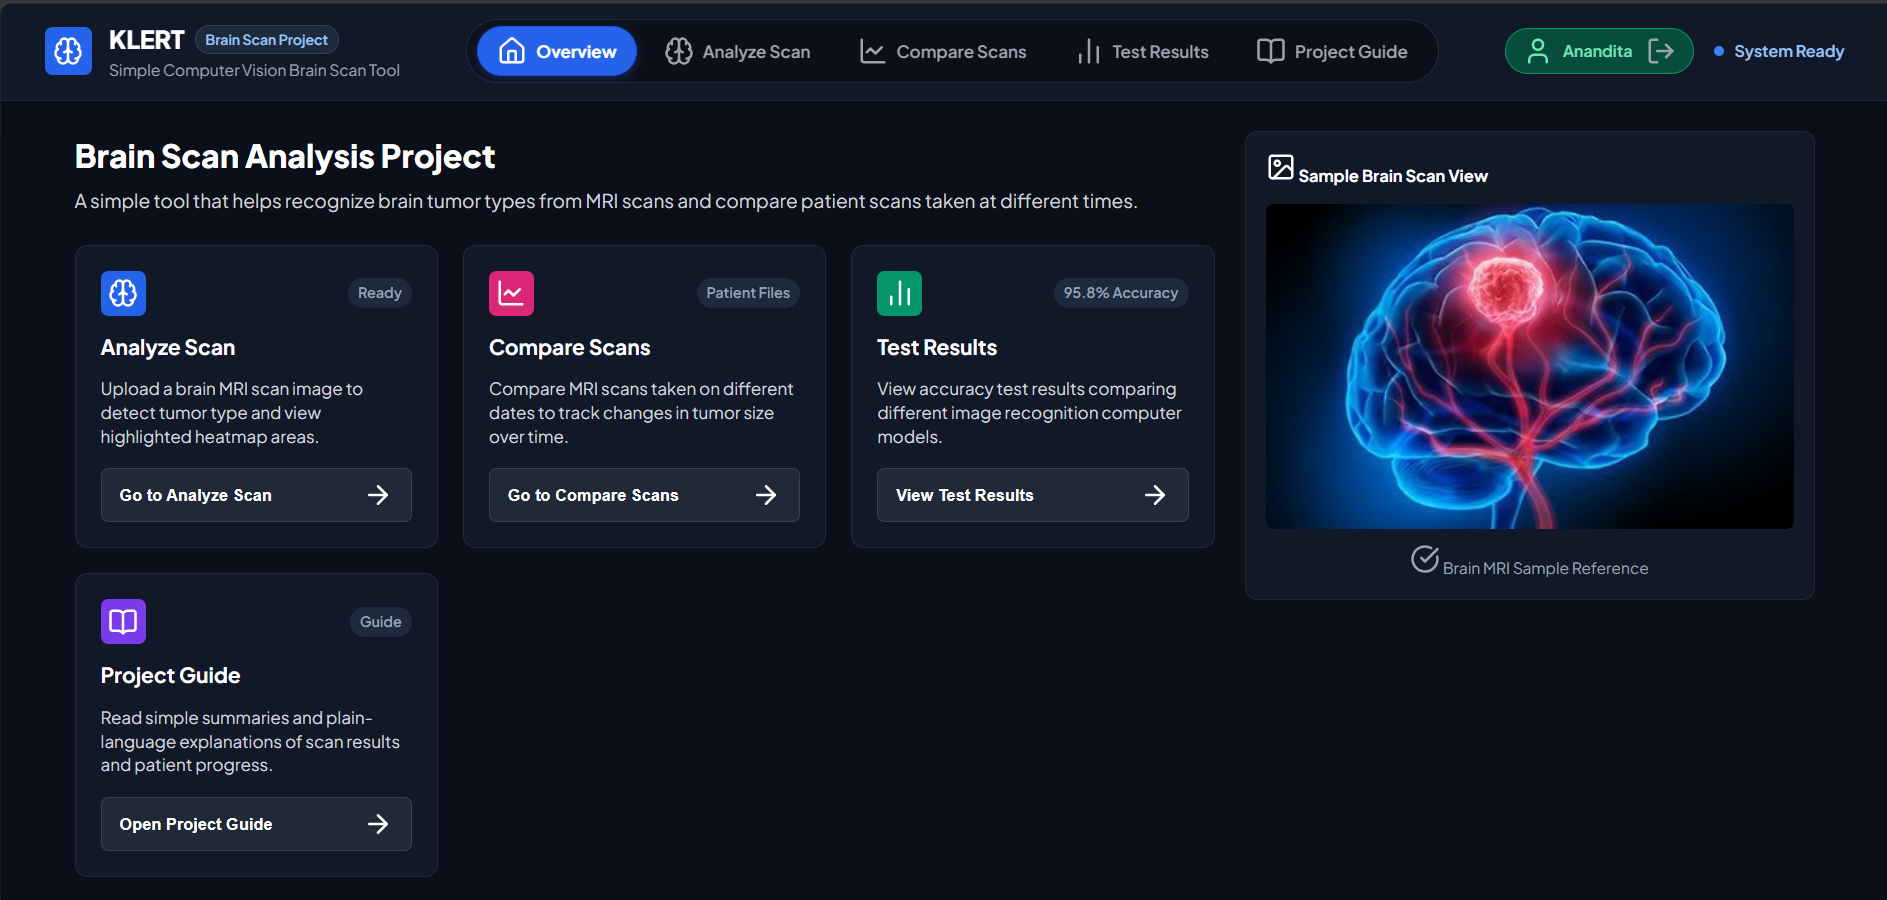
\includegraphics[width=\columnwidth]{klert-dashboard.png}
\caption{KLERT dashboard integrating scan analysis, comparison, evaluation, and project guidance.}
\label{fig:dashboard}
\end{figure}

For a valid image, the pipeline is:
\begin{equation}
\text{input} \rightarrow \text{validation} \rightarrow \text{preprocessing}
\rightarrow \text{inference} \rightarrow \text{explanation} \rightarrow \text{result}.
\end{equation}
For a DICOM study, the system additionally associates slices with their physical spacing and mask information. If $N$ mask voxels are active and $(d_x,d_y,d_z)$ are the voxel dimensions, the estimated volume is
\begin{equation}
V_{\mathrm{cm^3}} =
\frac{N d_x d_y d_z}{1000},
\label{eq:volume}
\end{equation}
where dimensions are expressed in millimetres. For baseline and latest volumes, the percentage change is
\begin{equation}
\Delta V(\%) =
\frac{V_{\mathrm{latest}}-V_{\mathrm{baseline}}}
{V_{\mathrm{baseline}}}\times 100.
\label{eq:change}
\end{equation}

\section{Implementation}
\subsection{Multi-Model Classification}
The custom BrainTumorCNN uses sequential convolutional blocks, nonlinear activation, pooling, dropout, and fully connected classification layers. ResNet-18 and VGG-16 provide pretrained comparison baselines. All models use a common input transformation and class ordering so their outputs can be compared in the same interface.

\subsection{Explainability}
For a selected class $c$, Grad-CAM computes channel weights from the gradient of the class score with respect to a convolutional feature map $A^k$:
\begin{equation}
\alpha_k^c = \frac{1}{Z}\sum_i\sum_j
\frac{\partial y^c}{\partial A_{ij}^k}.
\end{equation}
The explanation map is then
\begin{equation}
L_{\mathrm{Grad-CAM}}^c =
\mathrm{ReLU}\left(\sum_k \alpha_k^c A^k\right).
\end{equation}
The normalized map is resized and blended with the source scan, allowing the user to compare the evidence image with the prediction.

\begin{figure}[t]
\centering
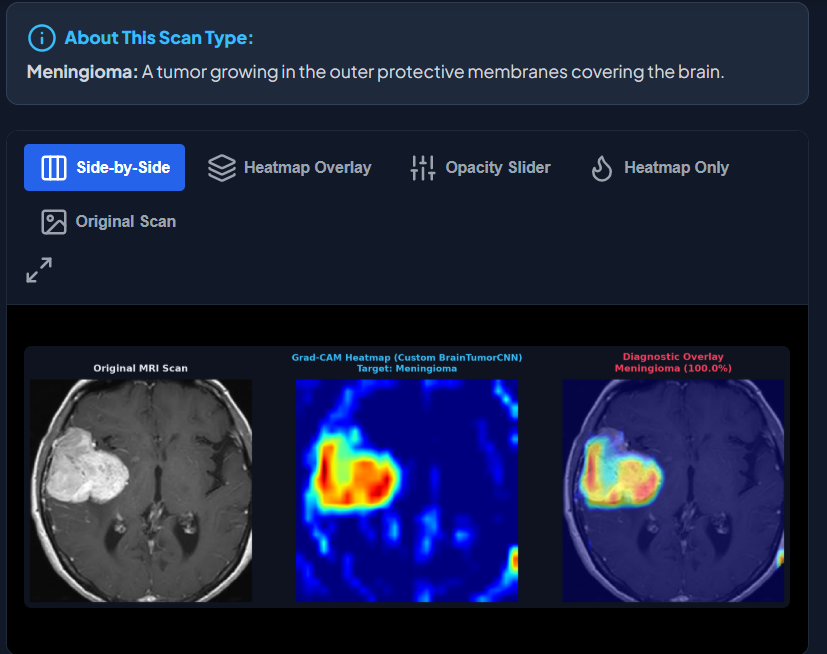
\includegraphics[width=\columnwidth]{klert-gradcam-result.png}
\caption{Grad-CAM result view showing the source MRI, activation heatmap, and diagnostic overlay.}
\label{fig:gradcam}
\end{figure}

\subsection{DICOM Progression and Clinical Summary}
The progression module reads compatible DICOM series, orders slices, applies available binary tumor masks, and computes volume for each study date. The interface presents baseline volume, latest volume, absolute change, and percentage change. An optional Gemini-based clinical agent converts structured outputs into a readable summary; generated text is advisory and is not a diagnosis.

\subsection{Web Service and Safety}
The service separates client interaction from model execution and validates uploaded files before processing. Dataset paths are resolved below an approved root to reduce path-traversal risk. Demonstration data should be de-identified, and deployment requires privacy review, access control, monitoring, prospective validation, and human oversight.

\section{Testing and Validation}
Testing covered the main user and service paths, including valid image upload, model switching, prediction rendering, Grad-CAM generation, DICOM parsing, volume comparison, invalid-file rejection, API response handling, concurrent requests, report generation, and responsive layout behaviour. The test matrix used twenty functional scenarios. The target was a complete, readable result for valid input and explicit error feedback for invalid input rather than a silent fallback.

\section{Results and Discussion}
The project evaluation used an independent test set of 1,311 brain MRI images. Table~\ref{tab:results} shows the reported benchmark.

\begin{table}[t]
\centering
\caption{Model performance benchmark}
\label{tab:results}
\begin{tabular}{lcccc}
\toprule
Model & Accuracy & Precision & Recall & F1-score\\
\midrule
BrainTumorCNN & 95.82\% & 96.10\% & 95.82\% & 95.74\%\\
ResNet-18 & 93.94\% & 94.36\% & 93.94\% & 93.82\%\\
VGG-16 & 92.25\% & 92.80\% & 92.25\% & 92.11\%\\
\bottomrule
\end{tabular}
\end{table}

The custom model produced the strongest aggregate result in this evaluation, while the additional models provide useful comparative context. A representative progression case decreased from $1.271$~cm$^3$ to $0.586$~cm$^3$, corresponding to a $-53.9\%$ change. Such a value is a computational summary of the supplied mask and scan metadata; it should not be interpreted without checking segmentation quality, acquisition consistency, and clinical context.

The primary benefit of the integrated design is traceability. A user can inspect the source image, class distribution, explanation map, and longitudinal measurement rather than receiving an unsupported label. Limitations include dependence on dataset quality, two-dimensional classifiers for the classification task, compatible segmentation masks for volume estimation, and network access for the optional language-model component.

\section{Conclusion and Future Scope}
KLERT demonstrates an end-to-end explainable medical-AI workflow for brain MRI classification and DICOM progression analysis. The combination of three classifiers, Grad-CAM explanations, physical-volume calculations, and a FastAPI web interface achieved a 95.82\% reported accuracy for the custom model and provided a structured basis for comparison and review.

Future work includes prospective multi-institution validation, calibrated uncertainty estimates, automated three-dimensional segmentation, PACS interoperability, privacy-preserving deployment, and evaluation with radiologists. These extensions are necessary before any clinical use.

\section*{Acknowledgment}
The author gratefully thanks the faculty and mentors at IIIT Naya Raipur for the teaching, guidance, and foundational knowledge gained there. What began as a 45-day journey of learning, building, experimenting, and debugging culminated in the development of the \textbf{AI-Powered Brain Tumor Identification and MRI Monitoring System}. The system supports AI-based brain-tumor classification from MRI scans, monitoring of tumor changes across scans acquired at different time points, AI-assisted identification and tracking of tumor-related changes, and interpretation of MRI results to support clinical decision-making.

\bibliographystyle{IEEEtran}
\bibliography{KLERT_CMES2027}

\end{document}
